\section{Experimental Validation}
\label{S:Exp}



\begin{figure*}[ht]
\centering
\subfigure[The test geometry, robot paths, and encounters (gray).]{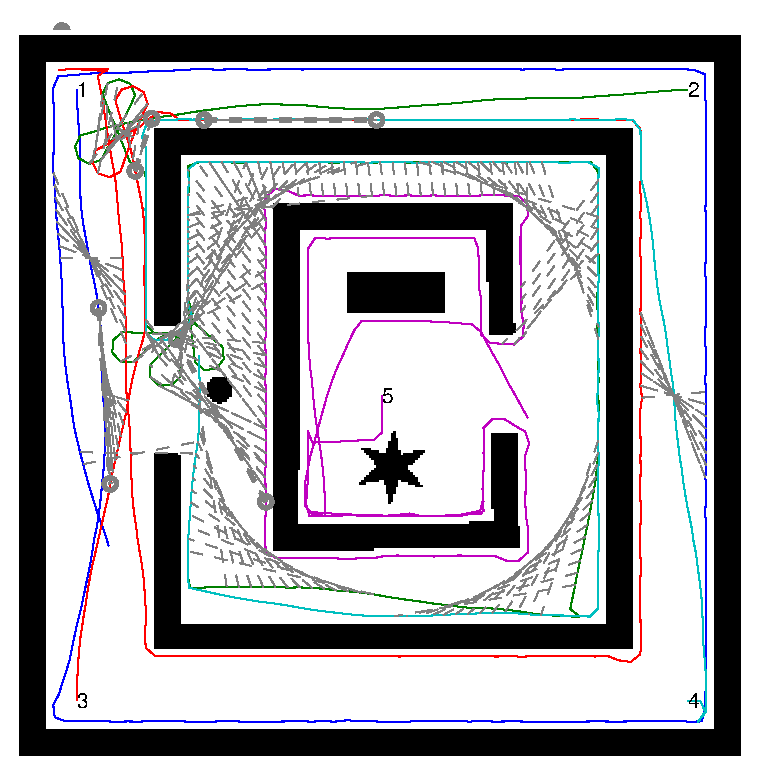
\includegraphics[width=\columnwidth]{../FinalFigures/Encounters}}
\subfigure[Robot encounters at a given time.]{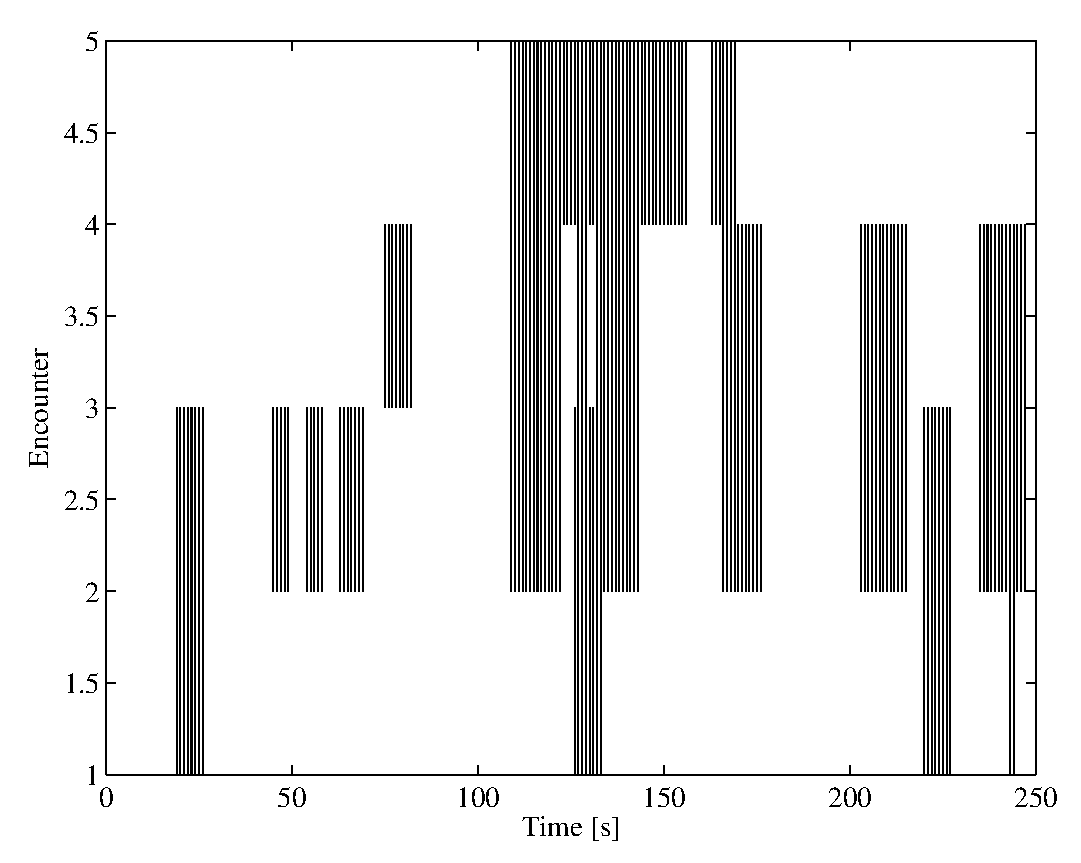
\includegraphics[width=\columnwidth]{../FinalFigures/EncountersTimes}}
\caption{}
\end{figure*}



\begin{equation}
\begin{bmatrix}
x_{t}\\
y_{t}
\theta_{t}
\end{bmatrix}=\begin{bmatrix}
x_{t-1}\\
y_{t-1}
\theta_{t-1}
\end{bmatrix}+\begin{bmatrix}
dx_t \cos(\theta_t+d\theta_t)\\
dy_{t}\sin(\theta_t+d\theta_t)\\
\theta_{t-1}+d\theta_t
\end{bmatrix}
\label{eq:OdometryMotion}
\end{equation}

\begin{figure}[ht]
\centering
\subfigure[Known Poses]{\includegraphics[width=\columnwidth]{../FinalFigures/KnownPoses}}
\subfigure[Pure Odometry]{\includegraphics[width=\columnwidth]{../FinalFigures/PureOdometry}}\\
\subfigure[Howard Implementation: Unknown Poses, low noise.]{\includegraphics[width=\columnwidth]{../FinalFigures/HowardLowNoise}}
\subfigure[Proposed Implementation: Unknown Poses, low noise.]{\includegraphics[width=\columnwidth]{../FinalFigures/OursLowNoise}}\\
\subfigure[Howard Implementation: Unknown Poses, High noise.]{\includegraphics[width=\columnwidth]{../FinalFigures/HowardHighNoise}}
\subfigure[Proposed Implementation: Unknown Poses, High noise.]{\includegraphics[width=\columnwidth]{../FinalFigures/OursLowNoise}}
\caption{Comparison between Howard's implementation and the proposed implementation.}
\end{figure}


